% 问题二正文；修改文字、公式与图表请直接编辑本文件。
\section{保证接收条件下的主动交会定位}\label{sec:q2}

一次示向度只能确定干扰源所在的狭长角域，沿示向方向移动虽然能够接近部分可能位置，却未必明显改善交会精度。
第二检测点的选择需要同时回答两个问题：到达该点后能否再次接收到信号，以及新增观测能否以较小移动代价缩小定位区域。
为此，先由首测信息构造保证接收的候选域，再在其中选择兼顾接近距离与残余不确定性的检测点。
本节建立的单源模块将在第三问中反复调用。

\subsection{首次观测与源位置可行域}\label{sec:q2-1}

记频道 \(f\) 的源坐标为 \(p\)，首个检测点为 \(x_1\)，测得示向度为 \(\theta_1\)；
目标区域为 \(\Omega=\{p:\|p\|\le1800\}\)。
接收半径 \(R_f\) 在单次测试中固定，但其数值未知，满足 \(R_{\min}=1000\le R_f\le R_{\max}=1500\)。
题面给出的测角误差界为 \(\varepsilon=1^\circ\)。
程序读取两位小数的角度时采用 \(\bar\varepsilon=1.005^\circ\)，额外的 \(0.005^\circ\) 用于保守容纳角度舍入，并非改变题设误差范围。

令 \(u(\alpha)=(\cos\alpha,\sin\alpha)\)，首测对应的前向角域为

\begin{equation}\label{eq:q2-1}
W(x_1,\theta_1)=\left\{p:
u(\theta_1-\bar\varepsilon)\times(p-x_1)\ge0,\quad
u(\theta_1+\bar\varepsilon)\times(p-x_1)\le0
\right\}.
\end{equation}

因此可保守保留

\begin{equation}\label{eq:q2-2}
C_f^{(1)}=\Omega\cap B(x_1,R_{\max})\cap W(x_1,\theta_1).
\end{equation}

其中 \(B(x,r)\) 表示闭圆盘。
获得示向度还意味着距离大于 \(5\) m；
省略这一个内圆排除能够保持凸性，只会扩大候选集。
实现时将两个圆约束换成外切正128边形，得到包含 \(C_f^{(1)}\) 的凸多边形 \(\widehat C_f^{(1)}\)。
以下选点与清除均依据该外包多边形，避免离散近似误删合法位置。
记 \(\rho(C)=\min_z\max_{p\in C}\|p-z\|\)，并以 \(z(C)\) 表示最小包围圆圆心。

\subsection{保证再次接收的第二点候选域}\label{sec:q2-2}

第二次检测若失去信号，便无法直接形成双站交会。
利用全向源的最小接收半径，定义

\begin{equation}\label{eq:q2-3}
Q_f=\bigcap_{p\in\widehat C_f^{(1)}}B(p,R_{\min})
=\left\{x:\max_{p\in\widehat C_f^{(1)}}\|x-p\|\le1000\right\}.
\end{equation}

对任意 \(x\in Q_f\)，真实源必有 \(\|x-p\|\le1000\le R_f\)，因而必然返回示向度或近场反馈。
若外包多边形顶点集合为 \(V_f\)，则

\begin{equation}\label{eq:q2-4}
Q_f=\bigcap_{a\in V_f}B(a,1000).
\end{equation}

证明只需利用凸性：任意 \(p=\sum_a\lambda_a a\) 满足 \(\|x-p\|\le\sum_a\lambda_a\|x-a\|\)。
所以检查全部顶点即能核验候选点，无须枚举区域内部。

该候选域并不要求预先知道源的距离。
外切128边形的最远顶点距离不超过 \(\widetilde R=R_{\max}\sec(\pi/128)\)，故忽略目标圆截断后，外包区域仍位于长度 \(\widetilde R\)、半角 \(\bar\varepsilon\) 的扇形内。
该扇形可被下列圆覆盖：

\begin{equation}\label{eq:q2-5}
z_0=x_1+\frac{\widetilde R}{2\cos\bar\varepsilon}u(\theta_1),
\qquad r_0=\frac{\widetilde R}{2\cos\bar\varepsilon}<1000.
\end{equation}

这是因为沿任一射线的距离平方关于径向坐标为凸函数，其最大值在径向两端取得，代入即可验证。
故 \(B(z_0,1000-r_0)\subseteq Q_f\) 是一个明确的安全候选子域；
考虑目标圆截断后，源的不确定性只会减小。
程序仍通过式\eqref{eq:q2-4}逐点重新核验候选位置。

式\eqref{eq:q2-3}给出容易计算的充分候选域，并非最大的保证接收域。
首测已接收还隐含 \(R_f\ge\|p-x_1\|\)，若联合保留源位置与接收半径，可进一步放宽部分检测点限制。
本方法使用统一的1000 m保证，以便在后续多次观测中直接复用。

\subsection{依据区域长轴构造有限探点}\label{sec:q2-3}

交会定位的一阶误差随两条视线夹角的正弦减小而放大。
因此，候选点既应包含沿首测方向接近区域的点，也应包含能够产生横向基线的点。
令 \(z=z(\widehat C_f)\)，当前位置为 \(x_0\)，首测方向的单位法向量为 \(n_1=(-\sin\theta_1,\cos\theta_1)\)。
先构造9个基础点：

\begin{equation}\label{eq:q2-6}
A_0=\{z\}\cup\left\{
x_0+t(z-x_0)+b n_1:
t\in\{1/2,1\},\ b\in\{-150,-50,50,150\}
\right\}.
\end{equation}

再取多边形最远顶点对的方向为单位长轴 \(e\)，其法向量为 \(e_\perp\)。
将所有顶点相对 \(z\) 投影到长轴，得到区间 \([\ell_-,\ell_+]\)，令 \(w=\ell_+-\ell_-\)、\(b_*=\min\{200,\max\{20,w/8\}\}\)。
补充

\begin{equation}\label{eq:q2-7}
\begin{aligned}
A_1={}&\{z+(\ell_-+tw)e+b e_\perp:
t\in\{1/4,3/8,5/8,3/4\},\ b\in\{-b_*,0,b_*\}\}\\
&\cup\{z-b_*e_\perp,z+b_*e_\perp\}.
\end{aligned}
\end{equation}

实现先在 \(A_0\) 中寻找满足式\eqref{eq:q2-4}的有效新点；
存在基础候选时，再扩展至 \(A_0\cup A_1\)。
删除重复点、同频道已测位置和不满足保证接收条件的点后，候选总数至多23个。
内侧的 \(3/8\)、\(5/8\) 位置有助于在首测角域较长、外侧探点难以保证接收时保留横向选择。
第二问中 \(x_0=x_1\)；
第三问则以当前实时位置和更新区域调用这一子程序。
后续多次定位若基础集合中已无合法新点，先尝试包围圆心及其180 m以内偏移点，再无新点则执行有限光学网格。
由于后续区域只收缩，式\eqref{eq:q2-5}保证其包围圆半径小于751 m，偏移回退点到任一可能源的距离小于 \(751+180<1000\) m，仍保持接收保证；
这一证明依赖区域更新正确且区域非空。

\subsection{有限名义观测下的选点评分}\label{sec:q2-4}

仅按移动距离选点可能保留过长的定位区域，仅追求区域最小又可能付出过大的绕行代价。
为同时反映这两方面，从当前区域选取至多5个名义源点：包围圆心 \(z\)，以及至多4个均匀抽取顶点沿连线向圆心移动四分之一所得的位置。
该集合记为 \(H_f=\{p^{(1)},\ldots,p^{(h)}\}\)，仅用于有限几何评价。

对于候选点 \(x\) 和名义源点 \(p^{(k)}\)，若二者距离大于5 m，则计算无附加误差的名义示向度，在区域副本中增加一次角度约束，得到残余半径 \(r_k(x)\)。
若距离不超过5 m，则按近场反馈处理。
取移动速度 \(v=5\) m/s、可靠清除门限 \(r_c=19.9\) m，定义

\begin{equation}\label{eq:q2-8}
\begin{aligned}
J(x)&=\frac{\|x-x_0\|}{v}
+\frac1h\sum_{k=1}^{h}\left[\frac{\|x-p^{(k)}\|}{v}+P_k(x)\right],\\
P_k(x)&=\begin{cases}
0,&\|x-p^{(k)}\|\le5,\\
6\,\mathbf1_{\{r_k(x)>r_c\}}
+\kappa\dfrac{(r_k(x)-r_c)_+}{v},&\text{其他情形},
\end{cases}\qquad\kappa=0.5.
\end{aligned}
\end{equation}

其中前两项衡量到探点及从探点接近名义源的移动代价；
6 s罚项近似反映仍需一次测量和换频的代价；
超出清除尺度的半径罚项抑制信息不足的探点。
对固定频道，当前检测及换频费用对所有候选相同，故不影响排序。
选择 \(J\) 最小的候选，并按横、纵坐标依次打破平局。
计算时先用不含非负罚项的部分建立下界，无法优于当前最优候选时提前停止该点评价。

等权名义点不代表已知的真实源后验分布，式\eqref{eq:q2-8}是有限代理目标，也不是所有误差下的最坏残余半径。
因此，本节得到的是可执行的主动选点策略；
有限候选的最小分值不等于连续候选域的全局最优。
执行第二次检测后，只用真实反馈更新 \(\widehat C_f\)，再计算实际残余半径。
若得到近场反馈，可在原位置清除；
否则，是否达到20 m清除要求须由更新区域重新判定。

\par\noindent\begin{minipage}{\linewidth}
\refstepcounter{algorithm}\label{alg:q2-probe}
\textbf{算法\thealgorithm：单源主动检测点选择}

\small
\textbf{输入：}当前点 \(x_0\)、首测方向 \(\theta_1\)、源外包区域
\(\widehat C_f\)、同频道历史测点。
\begin{enumerate}[label=\arabic*.,ref=\arabic*,leftmargin=2em,itemsep=2pt,topsep=4pt]
  \item 求 \(\widehat C_f\) 的包围圆心及长轴，先生成基础集合 \(A_0\)。
  \item 基础集合有有效新点时再扩展 \(A_1\)，去重并核验保证接收条件。
  \item 构造名义源点集合 \(H_f\)；对每个 \(x\in A\) 计算式\eqref{eq:q2-8}。
  \item 返回分值最小的 \(x\)；基础集合无新点时尝试圆心与偏移回退。
  \item 执行真实测量，以真实反馈更新区域或触发近场清除。
\end{enumerate}
\end{minipage}\par


\begin{figure}[!htbp]
\centering
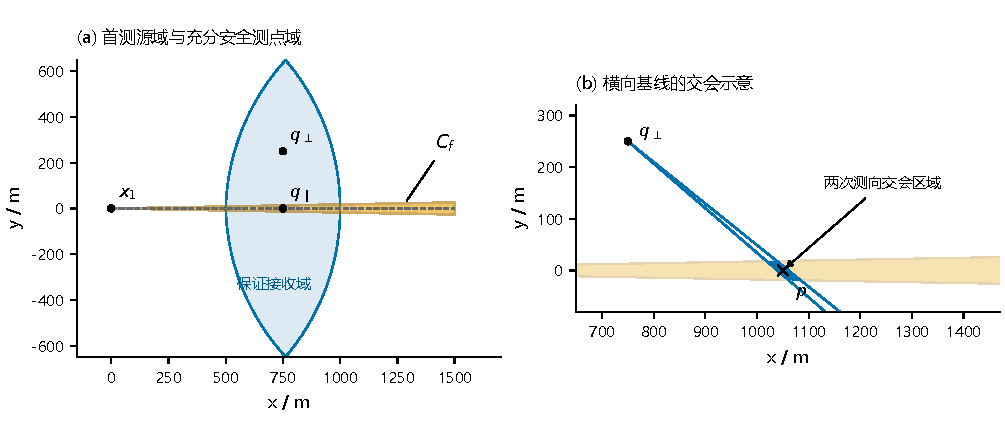
\includegraphics[width=\linewidth,height=\textheight,keepaspectratio,alt={首测可行域及横向交会的解析示意。半角采用1.005°，蓝色测点域由三角外包构造，属于充分保证接收域；示意源p仅用于解释交会几何，不作为规划输入。右图展示另一比例下的局部几何，不能作为算法性能比较。}]{figures/fig01_q2_geometry.pdf}
\caption{首测可行域及横向交会的解析示意。半角采用1.005°，蓝色测点域由三角外包构造，属于充分保证接收域；示意源p仅用于解释交会几何，不作为规划输入。右图展示另一比例下的局部几何，不能作为算法性能比较。}
\label{fig:q23-1}
\end{figure}

\subsection{真实观测算例}\label{sec:q2-5}

在场景800035的状态搜索轨迹中，按动作发生时间选择首个``同频道第二次有效示向来自主动定位''的实例，得到频道 20。
首测位于原点，第二测点由长轴分位候选策略实际选择；
此前该频道没有负观测或推断约束，因此使用这两次示向即可重建当时的全部源区域信息。

\Needspace{38mm}
\begin{center}
\begin{minipage}{\linewidth}
\centering\small
\captionof{table}{频道20的两次有效测量与区域收缩}
\label{tab:q2-example}
\vspace{4pt}
\begin{tabular}{@{}lcrr@{}}
\toprule
观测 & 检测点坐标 / m & 示向度 & 外包圆半径 / m \\
\midrule
原点首测 & (0.000, 0.000) & 125.00° & 750.226 \\
主动再测 & (-170.646, 568.027) & 148.14° & 65.012 \\
\bottomrule
\end{tabular}
\end{minipage}
\end{center}

两检测点相距 593.106 m。
第二点到首测外包区域各顶点的最大距离为 960.427 m，小于1000 m，满足保证再接收条件。
第二次观测将外包最小包围圆半径由750.226 m缩小至65.012 m，降幅约 91.33\%，但尚未达到19.9 m可靠清除门限，因此仍需后续观测或光学覆盖。
该例说明一次实际横向探测如何缩小可行域，不用于证明该选点优于所有其他候选。

重建沿用原评估版本的128边外切圆近似和1.005°计算半角；
题面误差界仍为1°，额外0.005°用于舍入余量。
算例仅由既有坐标和示向度重建，未使用真实源坐标选择实例；
原始动作及重建数值见辅助材料。

以上构造同时给出了第二检测点的候选区域与可执行选择规则。
其理论保证在于真实源保留、候选点可接收以及清除条件可靠；
选点效率仍须由实际后续测量检验。
本稿已有实验主要评估完整第三问，尚不把整局节省量当成第二检测点单独优越性的证据。
